\subsection{Setup version control for development project}
%\begin{itemize}
%    \item 2D game using 
%    \href{https://docs.godotengine.org/en/stable/getting_started/first_2d_game/index.html}{\color{blue}Godot 2D game instructions}
%    \item create empty godot project
%    \item setup workspace for version control with perforce and initial commit
%    \item follow development steps with version control
%\end{itemize}
The final step before the start of the development is to prepare the server depot and local workspace areas, connect 
and initialize them by adding the first version of files from the Godot project. 
The following section details the development steps of a very simple 2D game based on instructions from the Godot 
tutorial at \href{https://docs.godotengine.org/en/stable/getting_started/first_2d_game/index.html}{\color{blue}Godot 2D game instructions}
using Perforce's Helix Core as version control system.
\begin{enumerate}
    \item First, start by setting up a new depot on the server. Login to perforce. Run from terminal:
        \begin{verbatim}
            $ p4 login
            $ p4v
        \end{verbatim}
    \item Choose Tools {$=>$} Administration (or press CTRL+SHIFT+A). This brings up Helix Admin.
    \item From Helix Admin, File {$=>$} New {$=>$} Depot. Enter a name for the depot (\textit{godot2d} in my case), 
    choose stream as depot type then press \colorbox{blue!30}{OK}. The new empty depot is created on the server. 
    Finally, close Helix Admin.
    \item Create TypeMap. TypeMap tells Perforce how to treate different type of files and what rules should be applied
    on the type of files when being edited. E.g. some binary files cannot be modified if someone else is also working 
    on it as conflicts cannot be resolved and in such cases either one or the other version of the file has to be retained 
    and the other will be dropped. For these files, it is better to use the \textit{+l} modifier which automatically
    locks the file so multiple users are not allowed to edit the file at the same time.
    \begin{verbatim}
        TypeMap:
            binary //....meta
            binary+wS //....exe
            +l //project_a/....obj
    \end{verbatim}
    The '...' symbol is a recursive wildcard in Perforce ('*' is non-recursive wildcard).
    In this example, all files ending with .meta should be treated as binary, the .exe files should be treated as binary
    with the 'w' and 'S' modifiers (always writable and using latest revision), whereas all .obj files in the project\_a
    folder should be locked. To create a TypeMap, open a terminal and type the following command:
    \begin{verbatim}
        $ p4 typemap
    \end{verbatim}
    The command brings up a typemap template that is already defined for several file types. Unfortunately,
    the default editor for p4v is not the most user-friendly, so it makes sense to switch the editor before calling the
    previous command. To switch the editor to nano, type:
    \begin{verbatim}
        $ p4 set P4EDITOR=nano
    \end{verbatim}
    Now, it is much easier to make changes to the template typemap.
    The following typemap will be used for the project at hand:
    \begin{verbatim}
        Typemap:
            binary+lS //....png
            text+lS //....import
            text+w //....gd
            text+w //....tscn
            binary //....godot
    \end{verbatim}
    \item Next up, a stream is to be created. Streams are useful assets in Perforce as they allow different
    teams to work on the project without distracting each other. E.g. 3D modellers can work on one stream and developers 
    on another one and once they are both happy with the outcome, the development stream can be merged to the 3D modellers'
    stream to make the changes available to them. In this example, only one stream will be created.
    To do this, click the Add tab button on the right pane and select Stream Graph. Then right click in any blank space
    and select New stream. Populate the input fields: \\
    Stream name: main \\
    Stream type: mainline \\
    Depot: godot2d \\
    Uncheck Create Workspace and Populate checkbox to avoid these automatic steps. These will be executed manually.
    \begin{figure}[H]
        \centering
        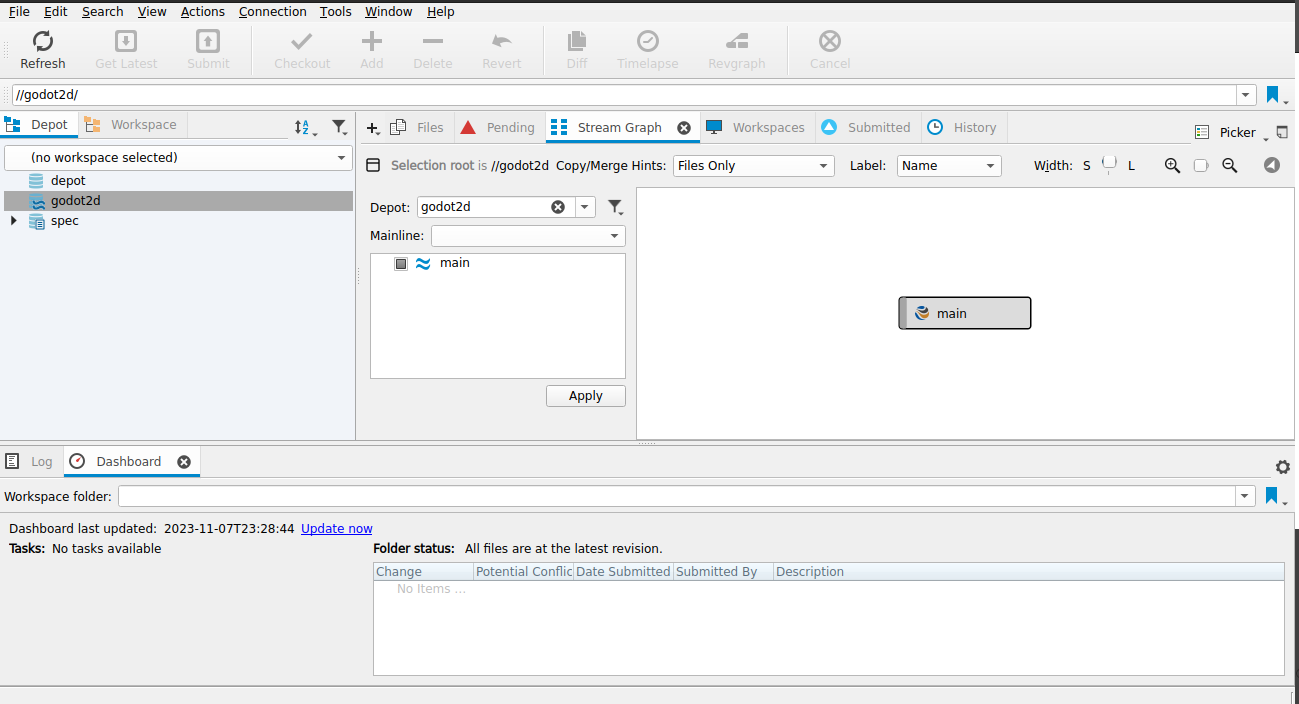
\includegraphics[width=\textwidth]{create-stream.png}
          \caption{new stream}
          \label{fig:new-stream}
    \end{figure}
    \item Next, a new workspace has to be created in p4v: click View {$=>$} Workspaces, right click on blank area on the
    right side when the Workspaces tab is active, click on new workspace. Instead of clicking, just press CTRL+N.
    \item Workspace name and root need to be given. The former usually follows the naming convention of 
    \textit{$<$user$>$\_$<$machine\_name$>$\_$<$project\_name$>$} which becomes in my case 
    \textit{super\_lefodor-HP\_godot2d}. The latter is set to any location on the local machine that ensures convenient
    working with the repository. Additionally, the stream is also to be filled out.
    \begin{figure}[H]
        \centering
        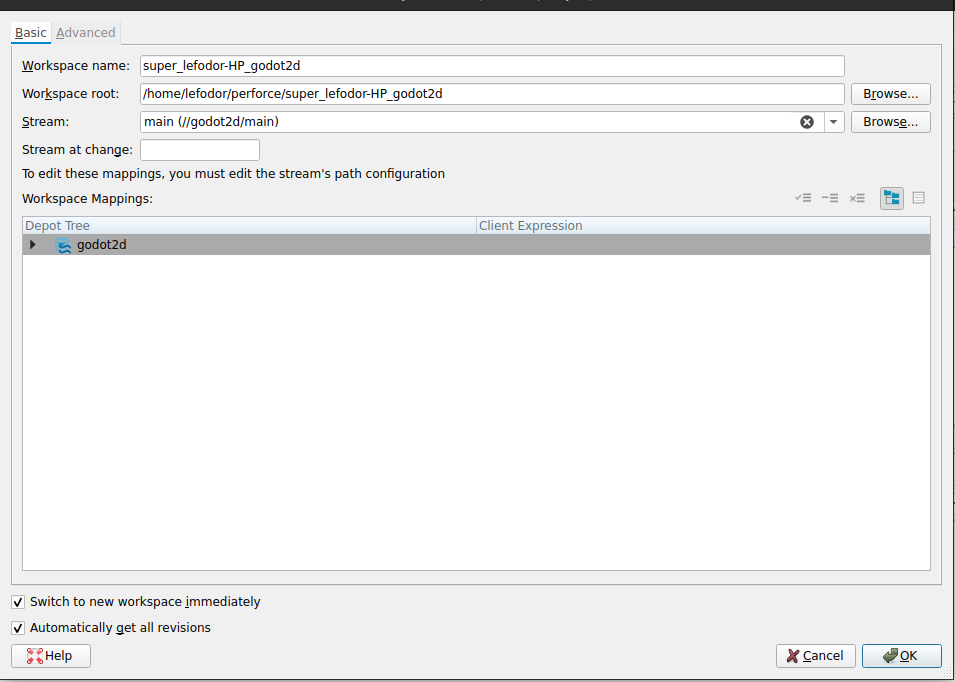
\includegraphics[width=\textwidth]{new-workspace2.png}
          \caption{new-workspace}
          \label{fig:new-workspace}
    \end{figure}
    Right click on all depots that are not required in the repository {$=>$} click Clear. After this step, only depot godot2d
    should have green pipe next to it. Then click on OK to create new workspace.
    \item Similarly to other version control systems, it is also possible to define a file that specifies files that are
    not subject to version control. In a new terminal window:
    \begin{verbatim}
        $ p4 set P4IGNORE=.p4ignore
        $ touch /home/lefodor/perforce/super_lefodor-HP_godot2d/.p4ignore
    \end{verbatim}
    In P4V, on the left pane right click on the file and click \textbf{Mark for Add} to add it to the default changelist, 
    and then hit \textbf{Submit} in the upper button bar while the file is selected.
    \item Add files to workspace. Copy blank Godot project folder to workspace root folder. Refresh P4V if needed to see
    the newly copied files in the left pane. Add the files to the default changelist and hit \textbf{Submit}. Only the 
    non-hidden files have been added to the workspace for version controll (note the small green icon next to files).
    \begin{figure}[H]
        \centering
        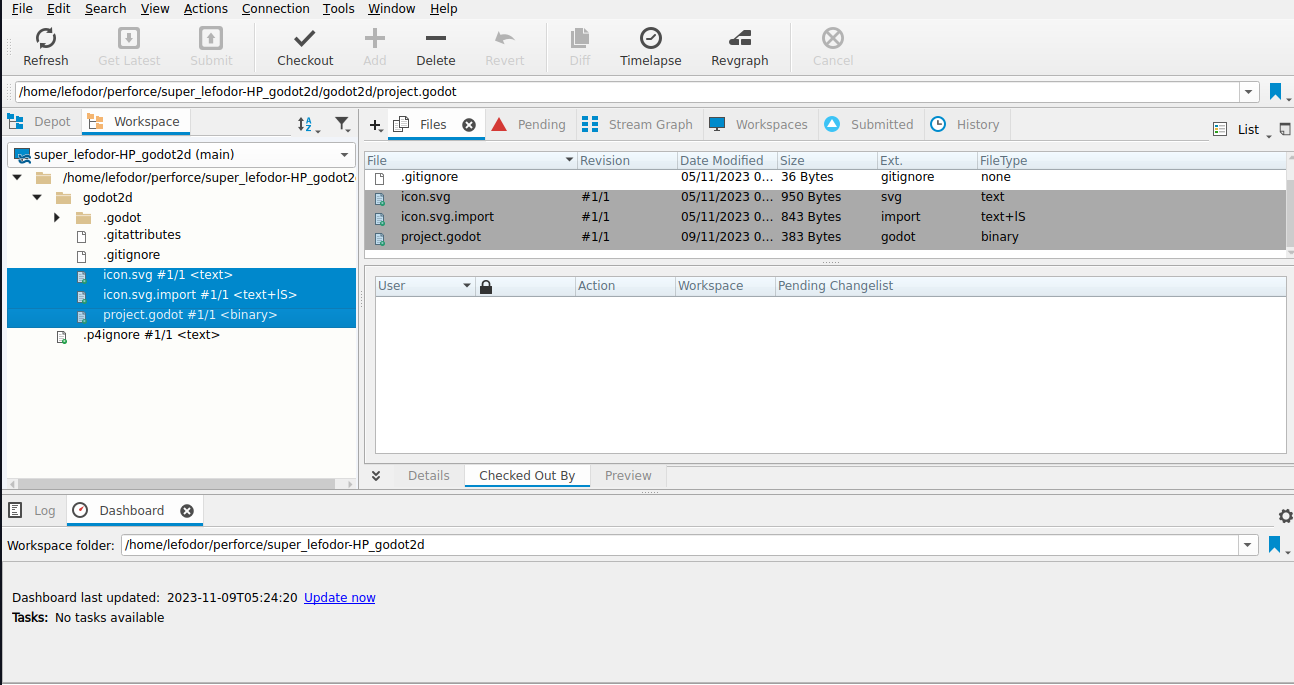
\includegraphics[width=\textwidth]{init-workspace.png}
          \caption{init-workspace}
          \label{fig:init-workspace}
    \end{figure}

    Having done the final step, the folder is ready to be shared and version controlled via the server depot and the 
    local workspace contents, currently 3 files are part of the repository of \textit{godot2d}.
\end{enumerate}
\subsection{First steps of game development}
Now, that the version control system, the game engine and the connections between the two are set up, the
development project can finally kick off. The steps in this sections are following the guide 
\href{https://docs.godotengine.org/en/stable/getting_started/first_2d_game/index.html}{\color{blue}Godot 2D game instructions}.
\begin{enumerate}
    \item Download assets and add them to version controll. Files are downloaded from 
    \href{https://github.com/godotengine/godot-docs-project-starters/releases/download/latest-4.x/dodge_the_creeps_2d_assets.zip}{\color{blue}here}.
    There are additional two more folders called \textit{art} and \textit{fonts} extracted and added to project folder.
    They need to be added to version control by selecting them, click \textbf{Add} button and then \textbf{Submit}.
    \begin{figure}[H]
        \centering
        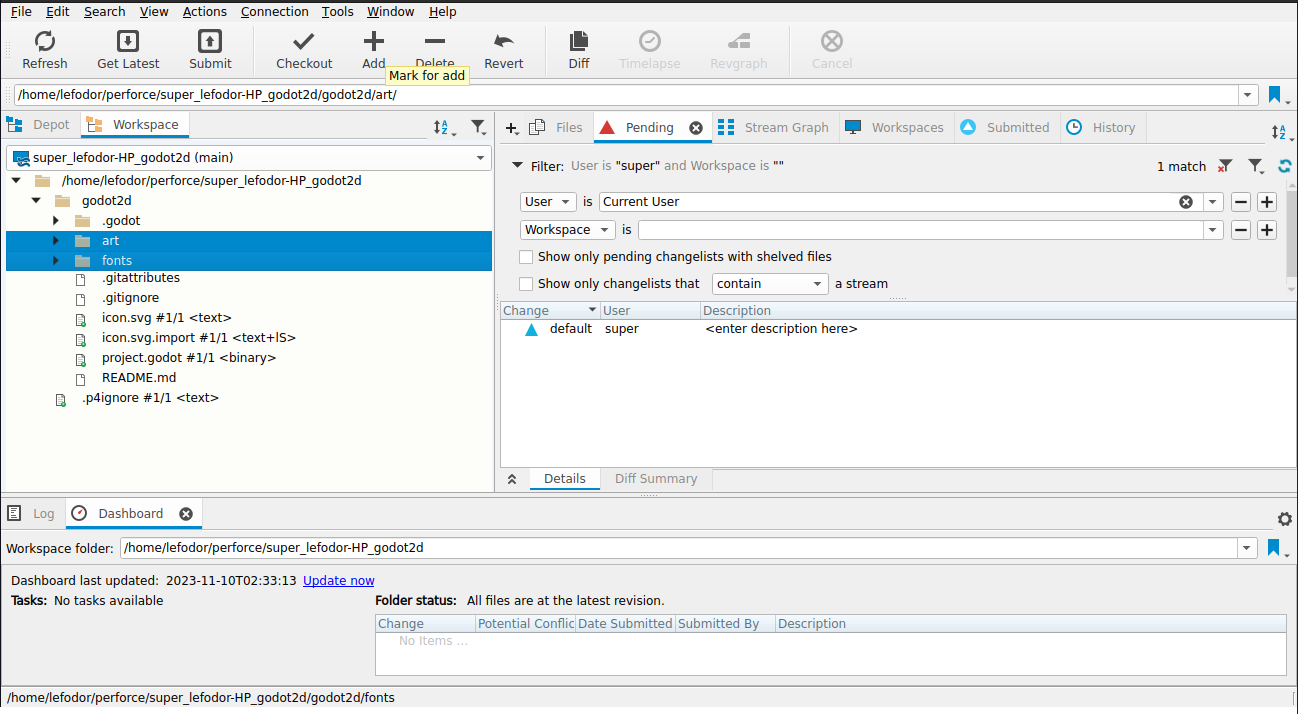
\includegraphics[width=\textwidth]{add-assets-to-vc.png}
          \caption{add assets to VC}
          \label{fig:add-assets-to-vc}
    \end{figure}
    \item Changes to \textit{.godot} project file
    \begin{itemize}
        \item Change project settings: click \textbf{Project} {$=>$} \textbf{Project Settings}. Under \textbf{Display/Window}
        change Viewport Width and Height to 480 and 720 respectively in the Size section and set Mode to \textit{canvas\_items}
        in Stretch section. In Perforce, the following changes can be observed: when \textit{godot2d} folder is checked out
        all the files are added to the changelist. When the changelist is submitted, new revision record shows up on the 
        right side pane, under History button. With right click on the revision, list of changed files can be opened (by
        clicking on \textit{View submitted changelist}) 
        \begin{figure}[H]
            \centering
            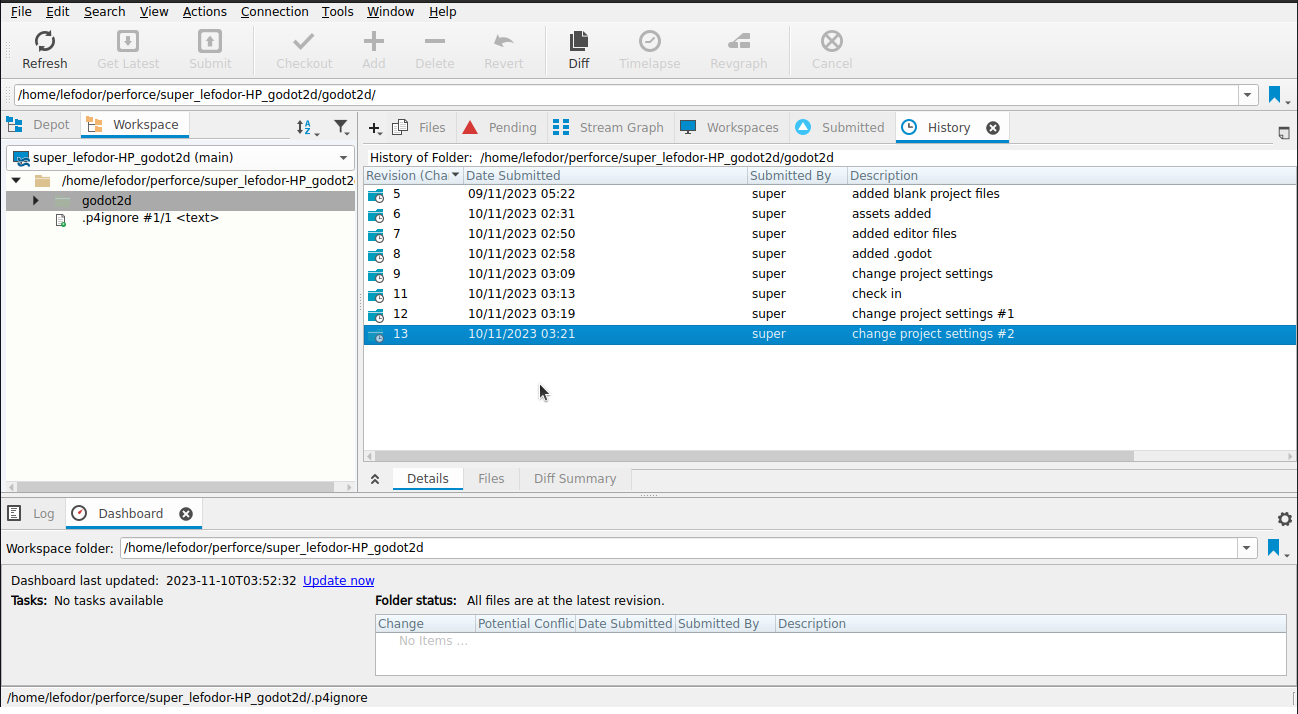
\includegraphics[width=\textwidth]{changes-in-perforce.png}
              \caption{project file changes in perforce}
              \label{fig:changes-in-perforce}
        \end{figure}
    \end{itemize}
    \item Create player scene. The player scene contains all objects related to the character controlled by the player.
    \begin{itemize}
        \item Click on \textbf{Other node} button and add an \textit{Area2D} node, rename it to player and save as 
        \textit{player.tscn}.
        \item \label{animation} Add sprite to player. Add a child node \textit{AnimatedSprite2D} to the player node and click the sprite frame
        property under \textit{Animation} section. Here, we can create 2 animations, the first is called 'up', and add 
        animation frames \textit{playerGrey\_up1.png} and \textit{playerGrey\_up2.png} from the downloaded asset folder.
        Secondly, add another animation called 'walk' with frames 
        \textit{playerGrey\_walk1.png} and \textit{playerGrey\_walk2.png}. Rescale by setting both x and y parameters under 
        \textit{Node2D/Transform} to 0.5.
        \item Add collision shape. Add a \textit{CollisionShape2D} as child node to player node. This will make possible
        for the character to collide with other objects. Select \textit{CapsuleShape2D} for shape property under 
        \textit{CollisionShape2D} at the right hand-side pane of the screen and adapt the size of the capsule on the 
        graphical interface so that it covers the animated sprite.
        \begin{figure}[H]
            \centering
            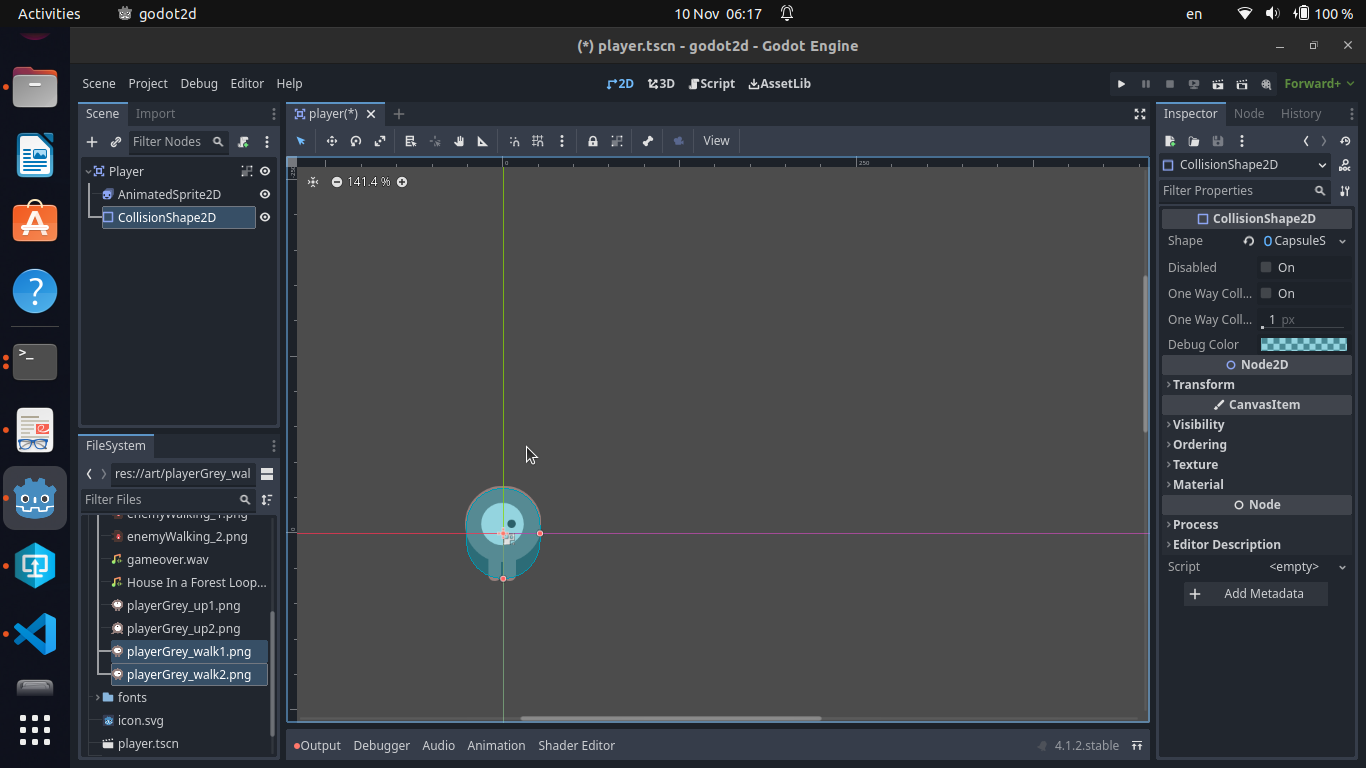
\includegraphics[width=\textwidth]{player-collision-shape.png}
              \caption{adding collision shape to player}
              \label{fig:player-collision-shape}
        \end{figure}
        \item After submitting in P4V, the changelist looks as follows for the above changes. Do not forget to add 
        the new \textit{player.tscn} file to the version controlled workspace.
        \begin{figure}[H]
            \centering
            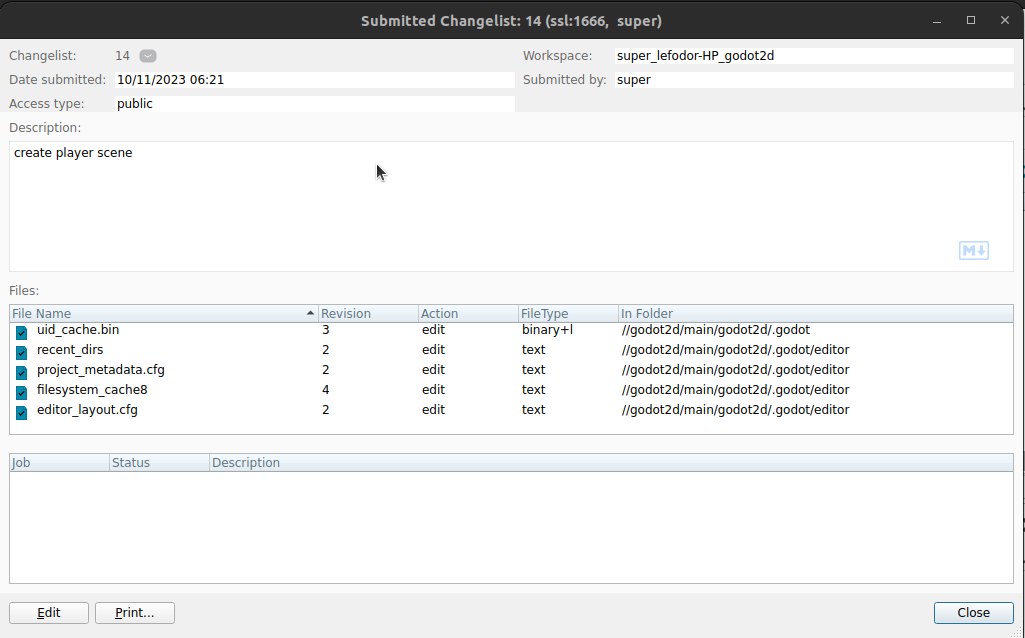
\includegraphics[width=\textwidth]{create-player-scene.png}
              \caption{p4v for create-player-scene}
              \label{fig:create-player-scene}
        \end{figure}
        \item More detailed steps can be found at 
        \href{https://docs.godotengine.org/en/stable/getting_started/first_2d_game/02.player_scene.html}{\color{blue}here}.
    \end{itemize}
\end{enumerate}